\documentclass{ximera}
\graphicspath{  %% When looking for images,
{./}            %% look here first,
{./pictures/}   %% then look for a pictures folder,
{../pictures/}  %% which may be a directory up.
{../../pictures/}  %% which may be a directory up.
{../../../pictures/}  %% which may be a directory up.
{../../../../pictures/}  %% which may be a directory up.
}

\usepackage{listings}
%\usepackage{circuitikz}
\usepackage{xcolor}
\usepackage{amsmath,amsthm}
\usepackage{subcaption}
\usepackage{graphicx}
\usepackage{tikz}
%\usepackage{tikz-3dplot}
\usepackage{amsfonts}
%\usepackage{mdframed} % For framing content
%\usepackage{tikz-cd}

  \renewcommand{\vector}[1]{\left\langle #1\right\rangle}
  \newcommand{\arrowvec}[1]{{\overset{\rightharpoonup}{#1}}}
  \newcommand{\ro}{\texttt{R}}%% row operation
  \newcommand{\dotp}{\bullet}%% dot product
  \renewcommand{\l}{\ell}
  \let\defaultAnswerFormat\answerFormatBoxed
  \usetikzlibrary{calc,bending}
  \tikzset{>=stealth}
  




%make a maroon color
\definecolor{maroon}{RGB}{128,0,0}
%make a dark blue color
\definecolor{darkblue}{RGB}{0,0,139}
%define the color fourier0 to be the maroon color
\definecolor{fourier0}{RGB}{128,0,0}
%define the color fourier1 to be the dark blue color
\definecolor{fourier1}{RGB}{0,0,139}
%define the color fourier 1t to be the light blue color
\definecolor{fourier1t}{RGB}{173,216,230}
%define the color fourier2 to be the dark green color
\definecolor{fourier2}{RGB}{0,100,0}
%define teh color fourier2t to be the light green color
\definecolor{fourier2t}{RGB}{144,238,144}
%define the color fourier3 to be the dark purple color
\definecolor{fourier3}{RGB}{128,0,128}
%define the color fourier3t to be the light purple color
\definecolor{fourier3t}{RGB}{221,160,221}
%define the color fourier0t to be the red color
\definecolor{fourier0t}{RGB}{255,0,0}
%define the color fourier4 to be the orange color
\definecolor{fourier4}{RGB}{255,165,0}
%define the color fourier4t to be the darker orange color
\definecolor{fourier4t}{RGB}{255,215,0}
%define the color fourier5 to be the yellow color
\definecolor{fourier5}{RGB}{255,255,0}
%define the color fourier5t to be the darker yellow color
\definecolor{fourier5t}{RGB}{255,255,100}
%define the color fourier6 to be the green color
\definecolor{fourier6}{RGB}{0,128,0}
%define the color fourier6t to be the darker green color
\definecolor{fourier6t}{RGB}{0,255,0}

%New commands for this doc for errors in copying
\newcommand{\eigenvar}{\lambda}
%\newcommand{\vect}[1]{\mathbf{#1}}
\renewcommand{\th}{^{\text{th}}}
\newcommand{\st}{^{\text{st}}}
\newcommand{\nd}{^{\text{nd}}}
\newcommand{\rd}{^{\text{rd}}}
\newcommand{\paren}[1]{\left(#1\right)}
\newcommand{\abs}[1]{\left|#1\right|}
\newcommand{\R}{\mathbb{R}}
\newcommand{\C}{\mathbb{C}}
\newcommand{\Hilb}{\mathbb{H}}
\newcommand{\qq}[1]{\text{#1}}
\newcommand{\Z}{\mathbb{Z}}
\newcommand{\N}{\mathbb{N}}
\newcommand{\q}[1]{\text{``#1''}}
%\newcommand{\mat}[1]{\begin{bmatrix}#1\end{bmatrix}}
\newcommand{\rref}{\text{reduced row echelon form}}
\newcommand{\ef}{\text{echelon form}}
\newcommand{\ohm}{\Omega}
\newcommand{\volt}{\text{V}}
\newcommand{\amp}{\text{A}}
\newcommand{\Seq}{\textbf{Seq}}
\newcommand{\Poly}{\textbf{P}}
\renewcommand{\quad}{\text{    }}
\newcommand{\roweq}{\simeq}
\newcommand{\rowop}{\simeq}
\newcommand{\rowswap}{\leftrightarrow}
\newcommand{\Mat}{\textbf{M}}
\newcommand{\Func}{\textbf{Func}}
\newcommand{\Hw}{\textbf{Hamming weight}}
\newcommand{\Hd}{\textbf{Hamming distance}}
\newcommand{\rank}{\text{rank}}
\newcommand{\longvect}[1]{\overrightarrow{#1}}
% Define the circled command
\newcommand{\circled}[1]{%
  \tikz[baseline=(char.base)]{
    \node[shape=circle,draw,inner sep=2pt,red,fill=red!20,text=black] (char) {#1};}%
}

% Define custom command \strikeh that just puts red text on the 2nd argument
\newcommand{\strikeh}[2]{\textcolor{red}{#2}}

% Define custom command \strikev that just puts red text on the 2nd argument
\newcommand{\strikev}[2]{\textcolor{red}{#2}}

%more new commands for this doc for errors in copying
\newcommand{\SI}{\text{SI}}
\newcommand{\kg}{\text{kg}}
\newcommand{\m}{\text{m}}
\newcommand{\s}{\text{s}}
\newcommand{\norm}[1]{\left\|#1\right\|}
\newcommand{\col}{\text{col}}
\newcommand{\sspan}{\text{span}}
\newcommand{\proj}{\text{proj}}
\newcommand{\set}[1]{\left\{#1\right\}}
\newcommand{\degC}{^\circ\text{C}}
\newcommand{\centroid}[1]{\overline{#1}}
\newcommand{\dotprod}{\boldsymbol{\cdot}}
%\newcommand{\coord}[1]{\begin{bmatrix}#1\end{bmatrix}}
\newcommand{\iprod}[1]{\langle #1 \rangle}
\newcommand{\adjoint}{^{*}}
\newcommand{\conjugate}[1]{\overline{#1}}
\newcommand{\eigenvarA}{\lambda}
\newcommand{\eigenvarB}{\mu}
\newcommand{\orth}{\perp}
\newcommand{\bigbracket}[1]{\left[#1\right]}
\newcommand{\textiff}{\text{ if and only if }}
\newcommand{\adj}{\text{adj}}
\newcommand{\ijth}{\emph{ij}^\text{th}}
\newcommand{\minor}[2]{M_{#2}}
\newcommand{\cofactor}{\text{C}}
\newcommand{\shift}{\textbf{shift}}
\newcommand{\startmat}[1]{
  \left[\begin{array}{#1}
}
\newcommand{\stopmat}{\end{array}\right]}
%a command to give a name to explorations and hints and theorems
\newcommand{\name}[1]{\begin{centering}\textbf{#1}\end{centering}}
\newcommand{\vect}[1]{\vec{#1}}
\newcommand{\dfn}[1]{\textbf{#1}}
\newcommand{\transpose}{\mathsf{T}}
\newcommand{\mtlb}[2][black]{\texttt{\textcolor{#1}{#2}}}
\newcommand{\RR}{\mathbb{R}} % Real numbers
\newcommand{\id}{\text{id}}
\newcommand{\coord}[1]{\langle#1\rangle}
\newcommand{\RREF}{\text{RREF}}
\newcommand{\Null}{\text{Null}}
\newcommand{\Nullity}{\text{Nullity}}
\newcommand{\Rank}{\text{Rank}}
\newcommand{\Col}{\text{Col}}
\newcommand{\Ef}{\text{EF}}
\newcommand{\boxprod}[3]{\abs{(#1\times#2)\cdot#3}}

\author{Zack Reed}
%borrowed from selinger linear algebra
\title{Application to Voting Records: A Need for Separation}
\begin{document}
\begin{abstract}

\end{abstract}
\maketitle


% ----------------------------------------------------------------------
\section*{Application to U.S. Senate voting data}

\subsection*{Setting up the problem: High-Dimensional Data}
The United States Senate%
\index{senate}%
\index{U.S. Senate}%
\index{United States Senate} votes on a lot of things: motions,
resolutions, amendments, and bills, among other things. Many of these
votes are roll call votes%
\index{voting}%
\index{roll call vote}, which means that the vote of every individual
senator is recorded (as opposed to a voice vote, where only the
outcome is recorded). Roll call data for the last 3 decades is
publicly available and can be downloaded from the U.S. Senate website
at \url{https://www.senate.gov/legislative/votes.htm}.

We will now explore how to use linear algebra to gain some useful information from the
voting records. The method of analysis that we will employ is central to this chapter, called {\bf \emph{principal component analysis}}.

The spreadsheet linked at the bottom of this page contains the votes of 99 senators for the first 200
roll call votes of 2007. Each row in the spreadsheet corresponds to a
senator, listed in alphabetical order from Daniel Akaka of Hawaii to
Ron Wyden of Oregon. I omitted one senator who died during 2007. Each
column of the spreadsheet corresponds to a vote. For example, the
first roll call vote of 2007 was on a resolution to honour President
Gerald Ford (it passed 88 to 0). Each cell of the spreadsheet contains
the number $1$ if the senator voted ``yes'', the number $-1$ if the
senator voted ``no'', and the number $0$ if the senator did not
vote. 
\begin{equation*}
  \begin{array}{|l|r|r|r|r|r|r|r|r}
    \hline
    \mbox{Akaka, Daniel (D) HI} & 1 & 1 & 1 & 1 & 1 & -1 & 1 & \ldots \\\hline
    \mbox{Alexander, Lamar (R) TN} & 0 & 1 & -1 & 1 & -1 & -1 & 1 & \ldots \\\hline
    \mbox{Allard, A. (R) CO} & 1 & 1 & -1 & -1 & -1 & 1 & 1 & \ldots \\\hline
    \mbox{Baucus, Max (D) MT} & 1 & 1 & 1 & 1 & 1 & -1 & 1 & \ldots \\\hline
    \mbox{Bayh, Evan (D) IN} & 1 & 1 & 1 & -1 & 1 & -1 & 1 & \ldots \\\hline
    \mbox{Bennett, Robert (R) UT} & 1 & 1 & -1 & 1 & 1 & -1 & 1 & \ldots \\\hline
    \mbox{\vdots} & \vdots & \vdots & \vdots & \vdots & \vdots & \vdots & \vdots & \ddots
  \end{array}
\end{equation*}
The human mind is not very well equipped to deal with such massive
amounts of data. Rather than listing 122 motions that Senator X
supported and 78 motions that she opposed, we like to come up with
abstractions, such as Senator X is ``conservative'', ``pro choice'',
``pro business'', ``hawkish'', etc. 

However, the problem with
abstractions is that they at best sometimes account for observed patterns in small subsets of data, or perhaps subsets that have value or meaning to the human experience, but can often fall very short of actually capturing true patterns in high-dimensional data. Luckily, we can use linear algebra to extract true patterns, separations, and variance in high-dimensional data. Moreover, we can explain these patterns using subspaces of impressively low dimension compared to the dimensionality of the data. 

We will represent each senator by a vector in $\R^{200}$, which
corresponds to a row of the above table. For example, to Senator
Akaka, we associate the vector
\begin{equation*}
  \startmat{c} 1 \\ 1 \\ 1 \\ 1 \\ 1 \\ -1 \\ 1 \\ \vdots \stopmat
  \in\R^{200}.
\end{equation*}
Thus, we can represent each senator (or more precisely, each senator's
voting record) as a point in 200-dimensional space. In this way, the
voting data can be interpreted as $99$ points in $\R^{200}$.

Unfortunately, 200 dimensions are impossible to visualize. But, as is thankfully the case with many real-world datasets, we actually need far fewer dimensions to make sense of our data. 

\subsection*{The Solution: Low-Dimensional Patterns}

Let's explore the solution to this issue with data that we can visualize. 

Open up MATLAB and load the \texttt{.mat} file called $\texttt{noise\_line.mat}$. Then take a look at the plot.

\begin{verbatim}

  load("+linalg/noisy_line.mat")
linalg.simple_plot_cloud(line_data);

\end{verbatim}

You should see an image like the following:

%855x641.25
\begin{center}
  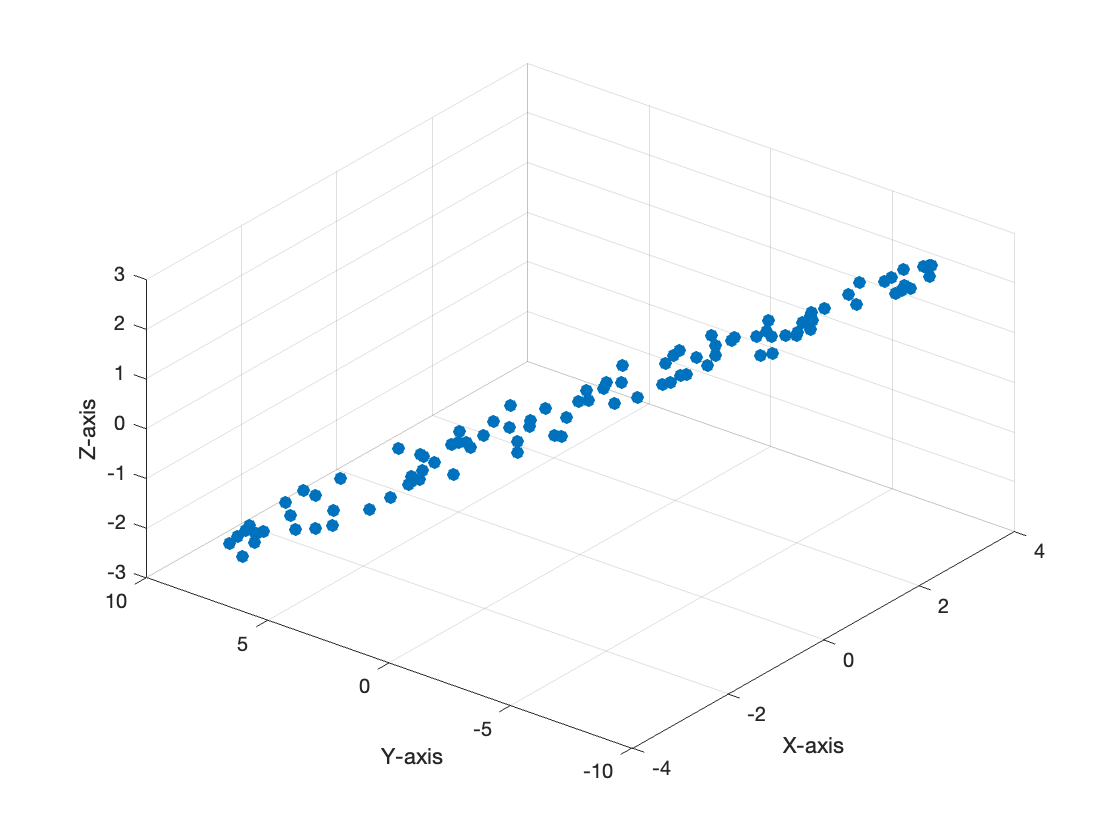
\includegraphics[width=22.62cm, height=17cm]{noisy_line_1.png}
\end{center}

The data is technically 3-dimensional, and it would be messy to try and make sense of the data from a table or from a single matrix, such as the following matrix showing the first 9 data vectors in 3D:

\[
\texttt{data\_matrix}=\begin{bmatrix}
-1.0201 & 3.0132  & -0.6987 \\
-0.3617 & 1.3268  & -0.3374 \\
2.0980  & -5.3478 & 1.2988  \\
-2.2879 & 6.4009  & -2.3206 \\
0.8898  & -1.9752 & 0.3144  \\
2.8387  & -7.7427 & 2.5059  \\
0.9423  & -2.5160 & 0.5328  \\
-2.5682 & 8.2888  & -2.5877 \\
1.3599  & -3.5429 & 1.1710\\
\ldots
\end{bmatrix}
\]

looking closely at the data, however, you might notice that the data is localized with a pseudo-linear relationship, generally moving up and to the right in 3D space. In fact, if you plot a line through the data, you notice that the datapoints don't stray too far from the line, as seen here:


\begin{center}
  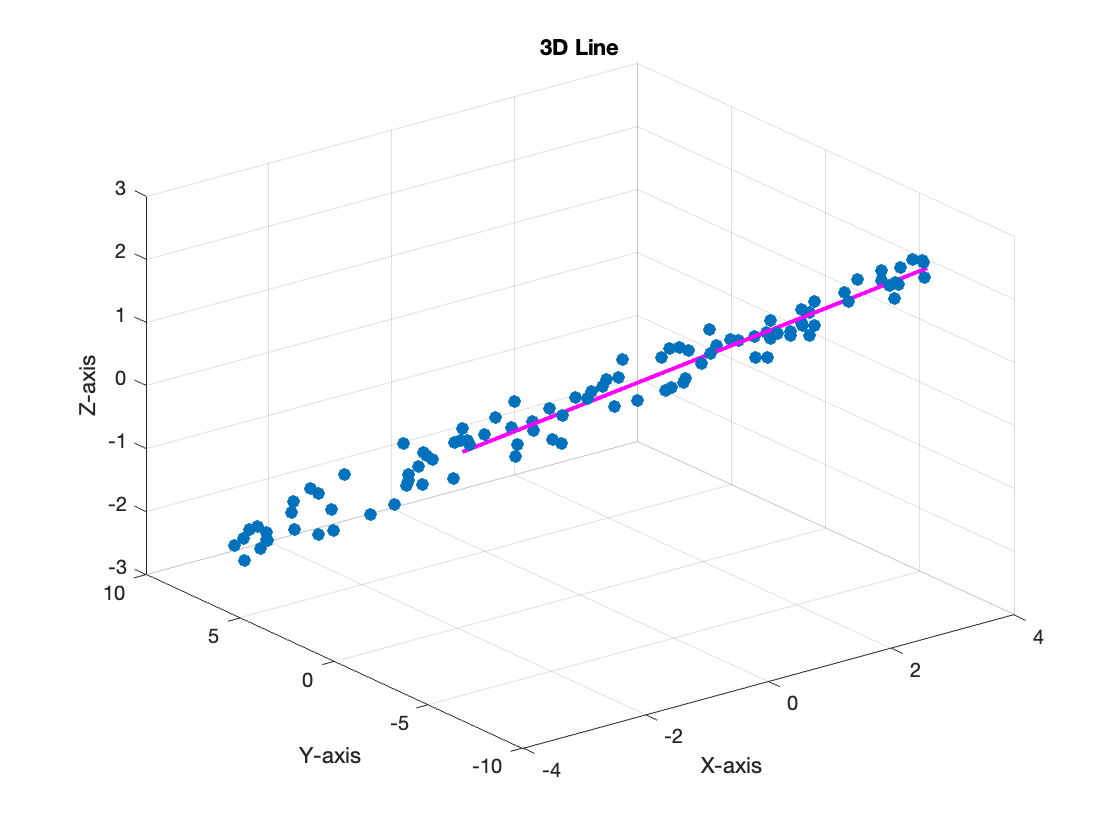
\includegraphics[width=22.62cm, height=17cm]{noisy_line_2.png}
\end{center}

Lines are $1$-dimensional vector spaces that can be described just by a point and a direction vector, which you can find from the loaded data as $\texttt{line\_point}$ and $\texttt{line\_direction}$. 

In some sense, this means that it is not too far off to describe the entire data set with just two vectors, $\texttt{line\_point}=\begin{bmatrix}0\\0\\0\end{bmatrix}$ and $\texttt{line\_direction}=\begin{bmatrix}.3180\\-.9090\\.2710\end{bmatrix}$. You might say that the data is comprised of points within the cube $[-4,4]\times[-10,10]\times[-3,3]$ that are ``close to'' the line $t\begin{bmatrix}.3180\\-.9090\\.2710\end{bmatrix}$. This is a much simpler description than the original data matrix. 

You might also gain information about regions or individual data points by determining the directions of data points along the line in relation to the center point, in this case $\vec{0}$. For instance, if you project the data points onto the line, you can separate the data into two groups determined by their location relative to the center point. 

Try the following:

\begin{verbatim}

  projection_magnitudes=line_data'*line_direction
  projections=projection_magnitudes*line_direction'
  linalg.simple_plot_cloud(projections');

\end{verbatim}

You should see the following line, which is the projections of the data points along the line.

\begin{center}
  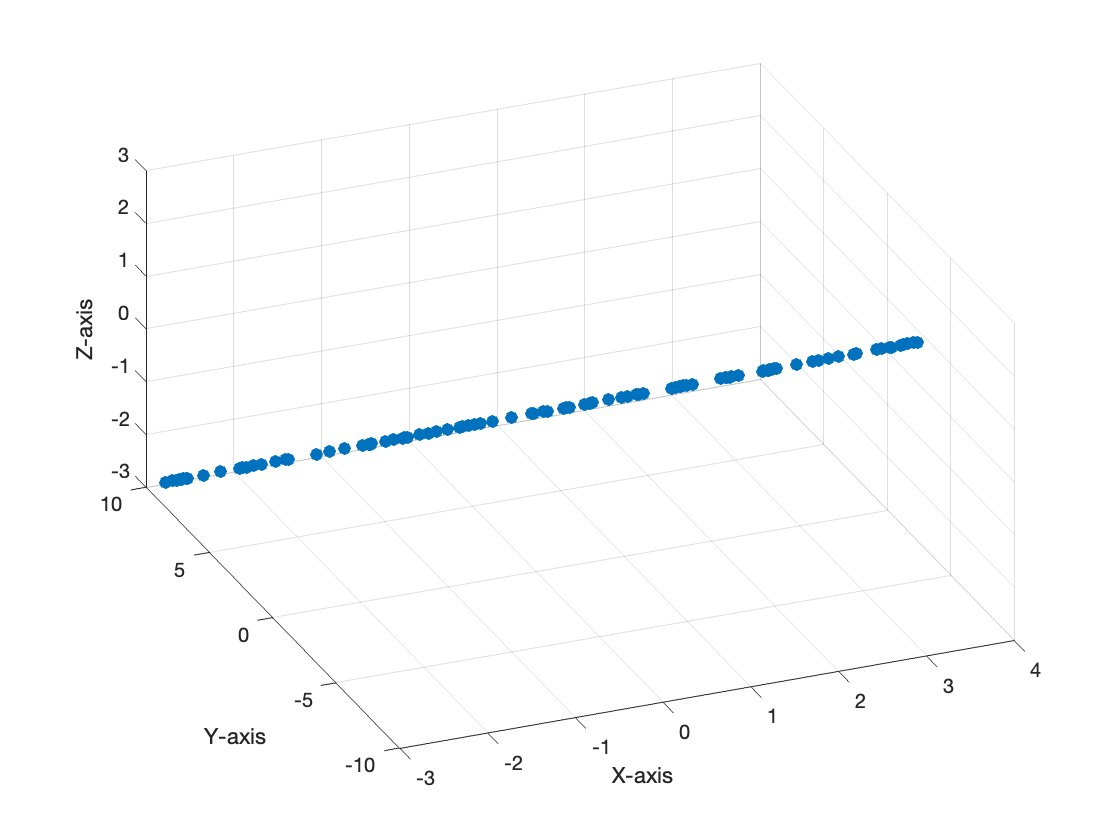
\includegraphics[width=22.62cm, height=17cm]{noisy_line_projections.png}
\end{center}

You can then separate the points along the center, by creating "left" and "right" sets and plotting them individually.

\begin{verbatim}

  greater=find(projection_magnitudes>=0)
  less=find(projection_magnitudes<0)
  right=projections(greater,:)
  left=projections(less,:)
  linalg.simple_plot_cloud(left',right');

\end{verbatim}

You should see a color-separated plot like this:

\begin{center}
  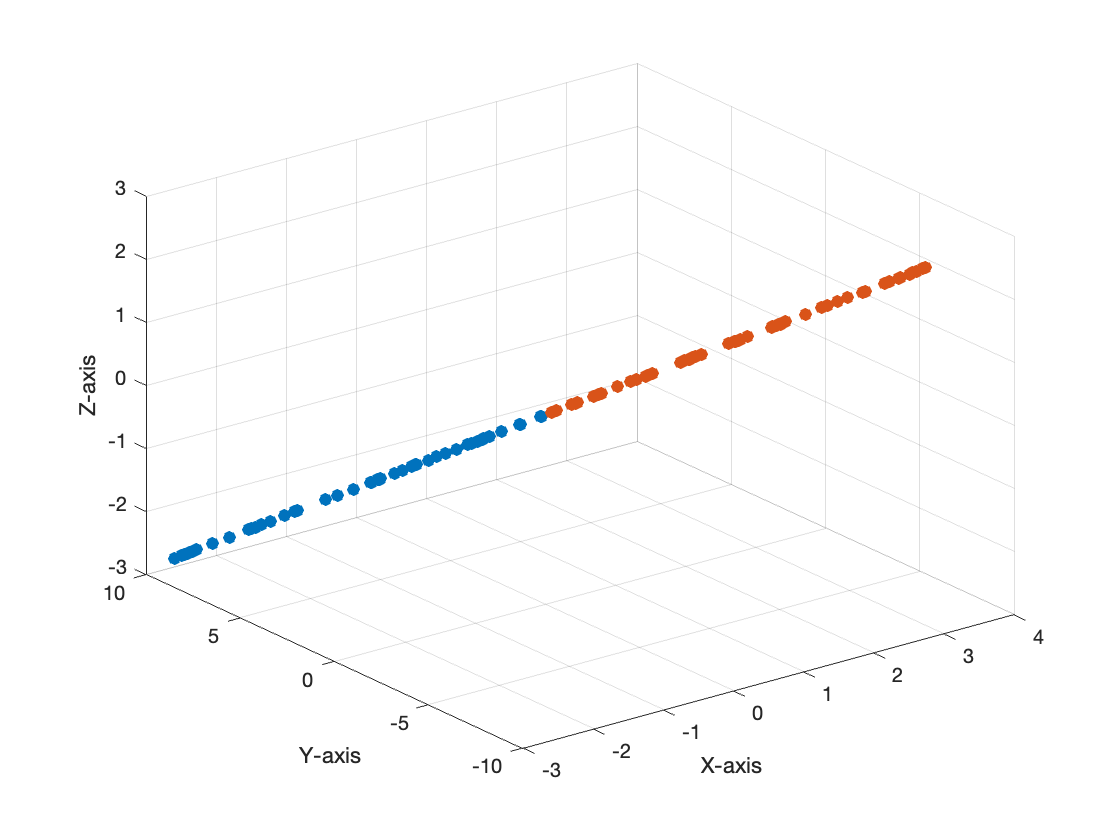
\includegraphics[width=22.62cm, height=17cm]{noisy_line_separated.png}
\end{center}

This brief (and somewhat simplistic) analysis relied on the fact that the $3$-dimensional data was pretty close to a $1$-dimensional subspace, a line, which we could then exploit to reduce the complexity of the data while preserving the important characteristics of the data. 

This is an example of what is called {\bf \emph{principle component analysis}}. In the sections that follow, we will examine what it means to be ``close'' to these smaller-dimensional hyperplanes of high-dimensional space, and how we find these useful lower-dimensional subspaces. 

Now, we'll perform a similar analysis and breakdown of the Senate Voting data.

\subsection*{Applying PCA to Voting Data}

What if, like the ``noisy-line'' data,
the voting records of all the senators lie on (or at least close to) a
much-smaller-dimensional subspace (after centering)? This is actually not an
unreasonable expectation; after all, there are probably only a handful
of issues most senators care about. For example, if a certain senator
supports gun control, he will be likely to vote a certain way on
measures that affect gun control. If another senator supports the gun
lobby, she is likely to vote the opposite way.

We can thus analyze the 
problem as follows: we are looking for a low-dimensional subspace, centered around an average location, that is
close to all $99$ points. 

We call this ``centering location" of our subspace the \emph{centroid} of the data. If you think about data as a cloud in 3-dimensional space, this is akin to finding the center of mass. In practice, the centroid is the average of the data vectors. 

Then, using software, we can find the directions within our 200-dimensional space that best describe our voting data.

%find the
%eigenvalues and -vectors of $B$. The first few eigenvalues (in
%decreasing order) are:
%\begin{equation*}
%  \eigenvar_1 = 7255.65,\quad
%  \eigenvar_2 = 519.16,\quad
%  \eigenvar_3 = 430.60,\quad
%  \eigenvar_4 = 278.05,\quad\mbox{and}\quad
%  \eigenvar_5 = 230.56.
%\end{equation*}
%All of the remaining eigenvalues are less than $200$, and the sum of
%the remaining eigenvalues is
%$\eigenvar_6+\ldots+\eigenvar_{200}=3913.46$. 

For reasons that we will explore later, the vast
majority of the voting behavior of each senator is determined by a
single dimension %given by the eigenvector corresponding to the
%eigenvalue $\eigenvar_1$. In other words, there is a $1$-dimensional
%affine subspace that all $99$ points are pretty close to. If we
%project each senator to this affine subspace, we get the following
%picture:

%111.76x44.17

If we plot along the line given by this direction vector (taken from the centroid), we get the following separation of senators:

\begin{center}
  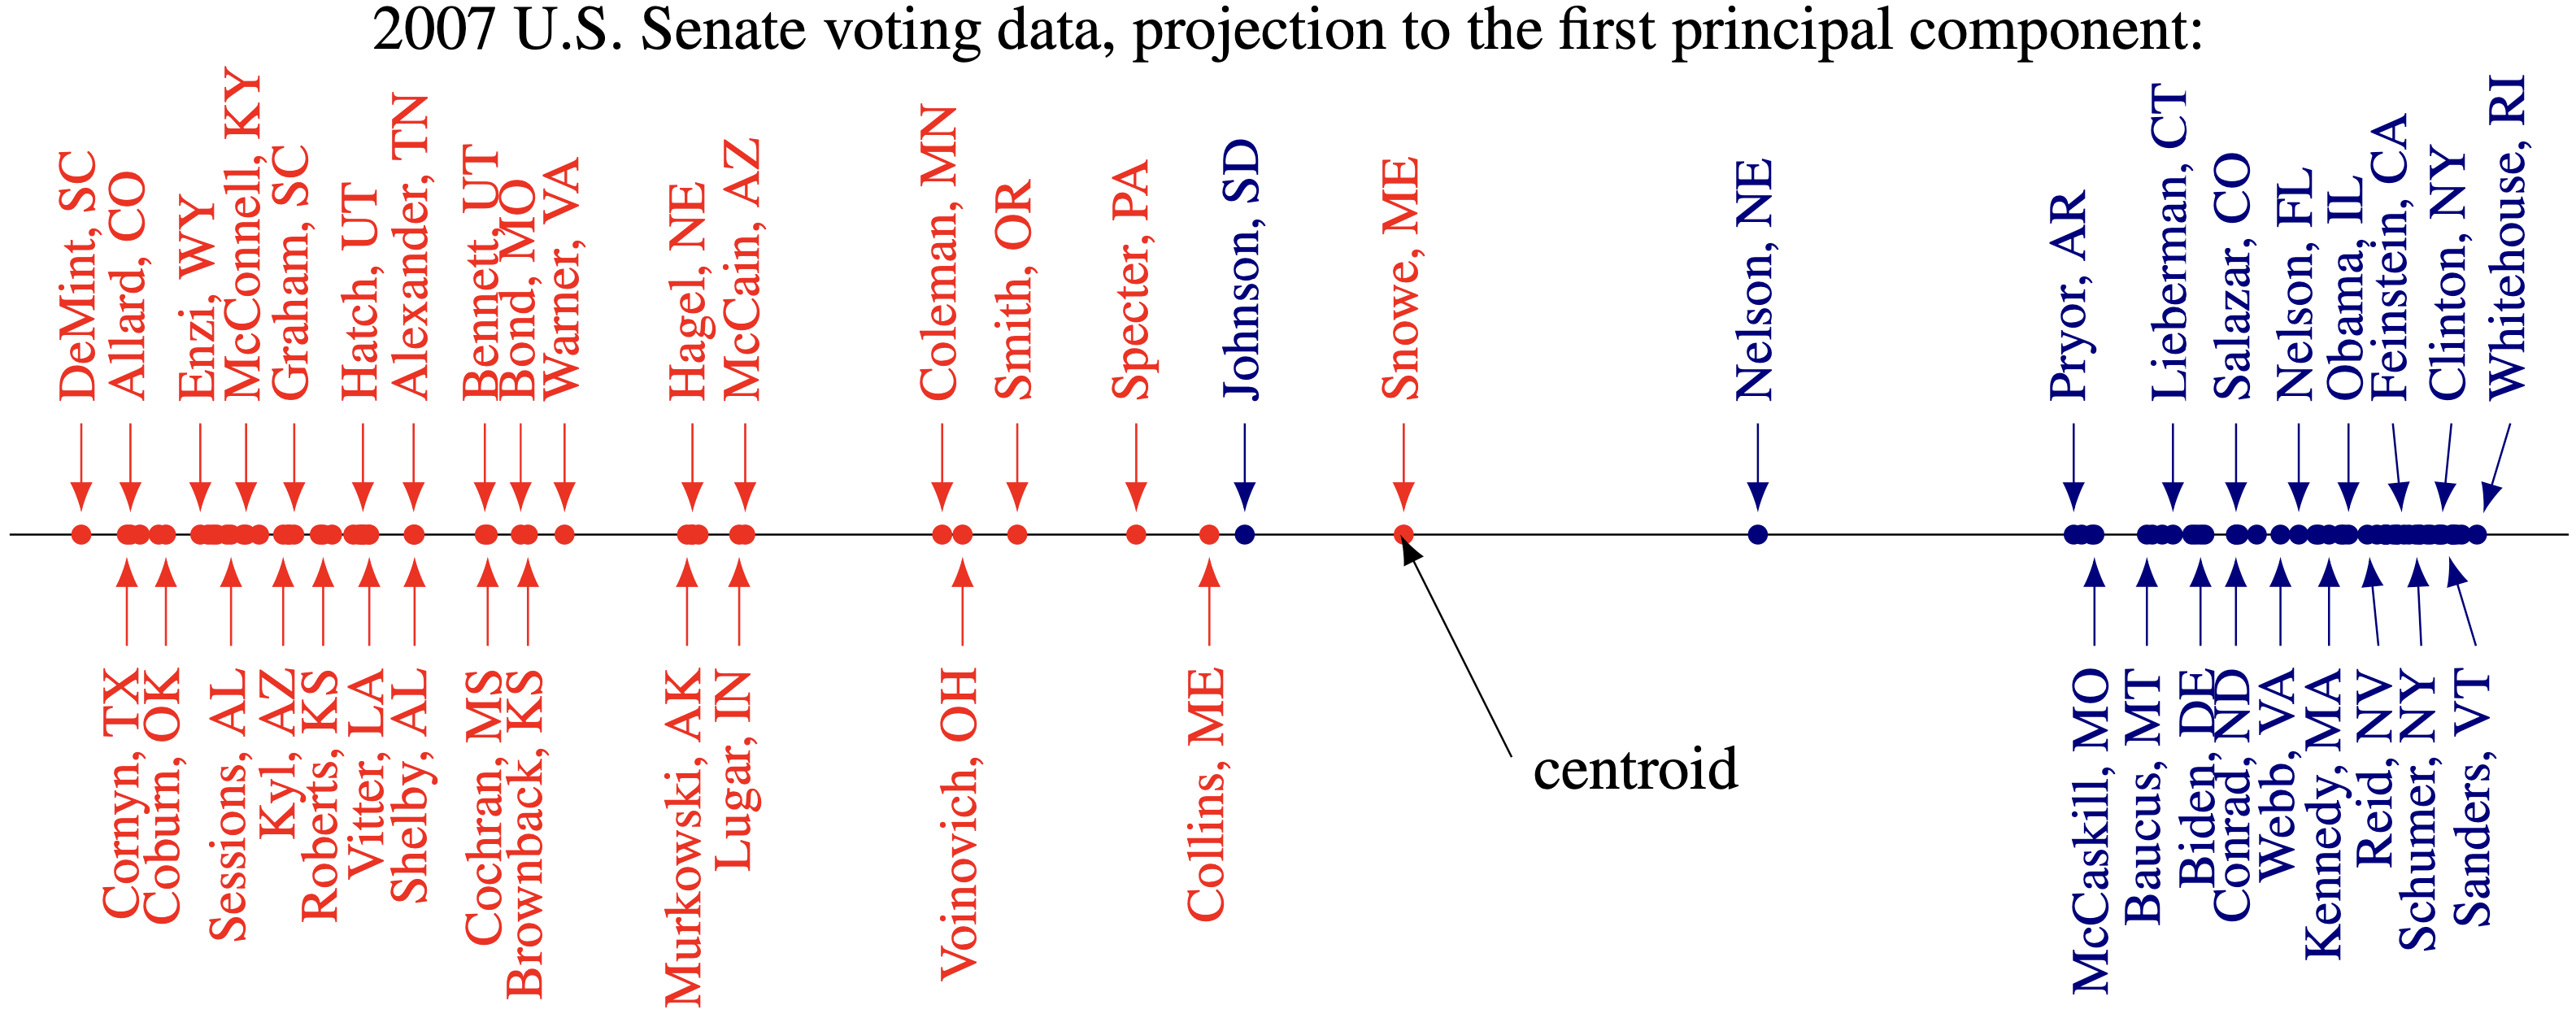
\includegraphics[width=31.93cm, height=12.62cm]{pca_senate_1.png}
\end{center}

For convenience, Republican senators have been shown in red and
Democratic and independent senators in blue. Not all senators have
been named, because in some areas they are clustered very densely. 

An
interpretation of the principal component then immediately suggests
itself: it appears to be the ``conservative'' vs. ``liberal'' axis. We
can use this picture to assist in answering questions such as: {\em
  ``Which party votes more uniformly?''}, {\em ``Which state are the
  most liberal Republicans from?''}, {\em ``Which states are the most
  conservative Democrats from?''}, {\em ``Was Obama really a
  radical?''}, and {\em ``Was McCain really a maverick?''}.  If we
repeat the same calculation for the 2017 senate, we get the following
picture:

%112.96x44.87
\begin{center}
  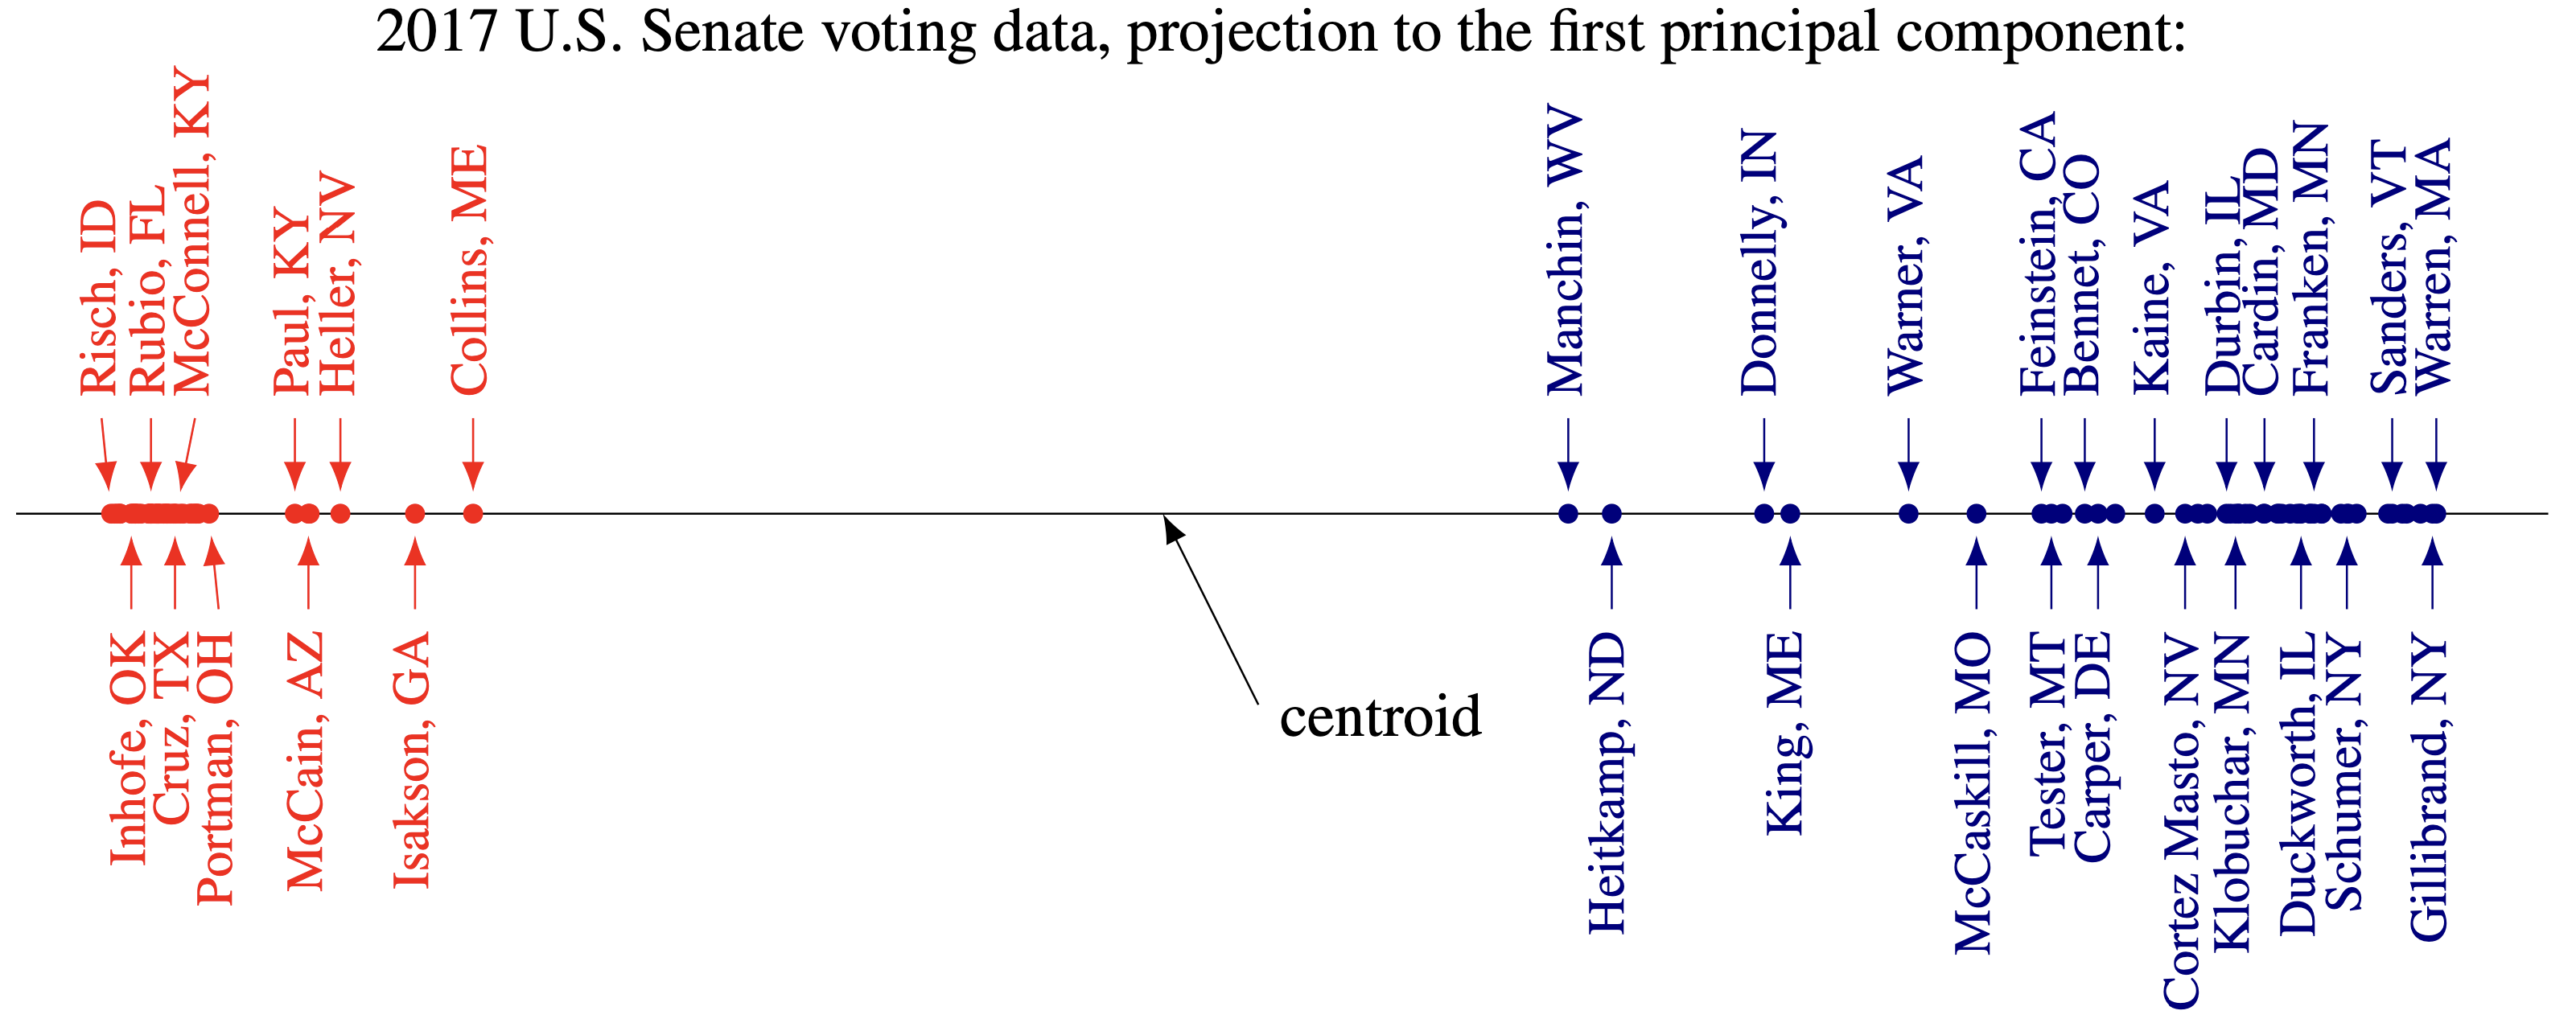
\includegraphics[width=32.27cm, height=12.82cm]{pca_senate_2.png}
\end{center}

We can use this to help answer questions such as {\em ``Has the senate
  become more partisan between 2007 and 2017?''}.

If we instead project the data onto a $2$-dimensional subspace that best explains the data variety, we get the following picture for the 2007 data:

%115.71x75.21
\begin{center}
  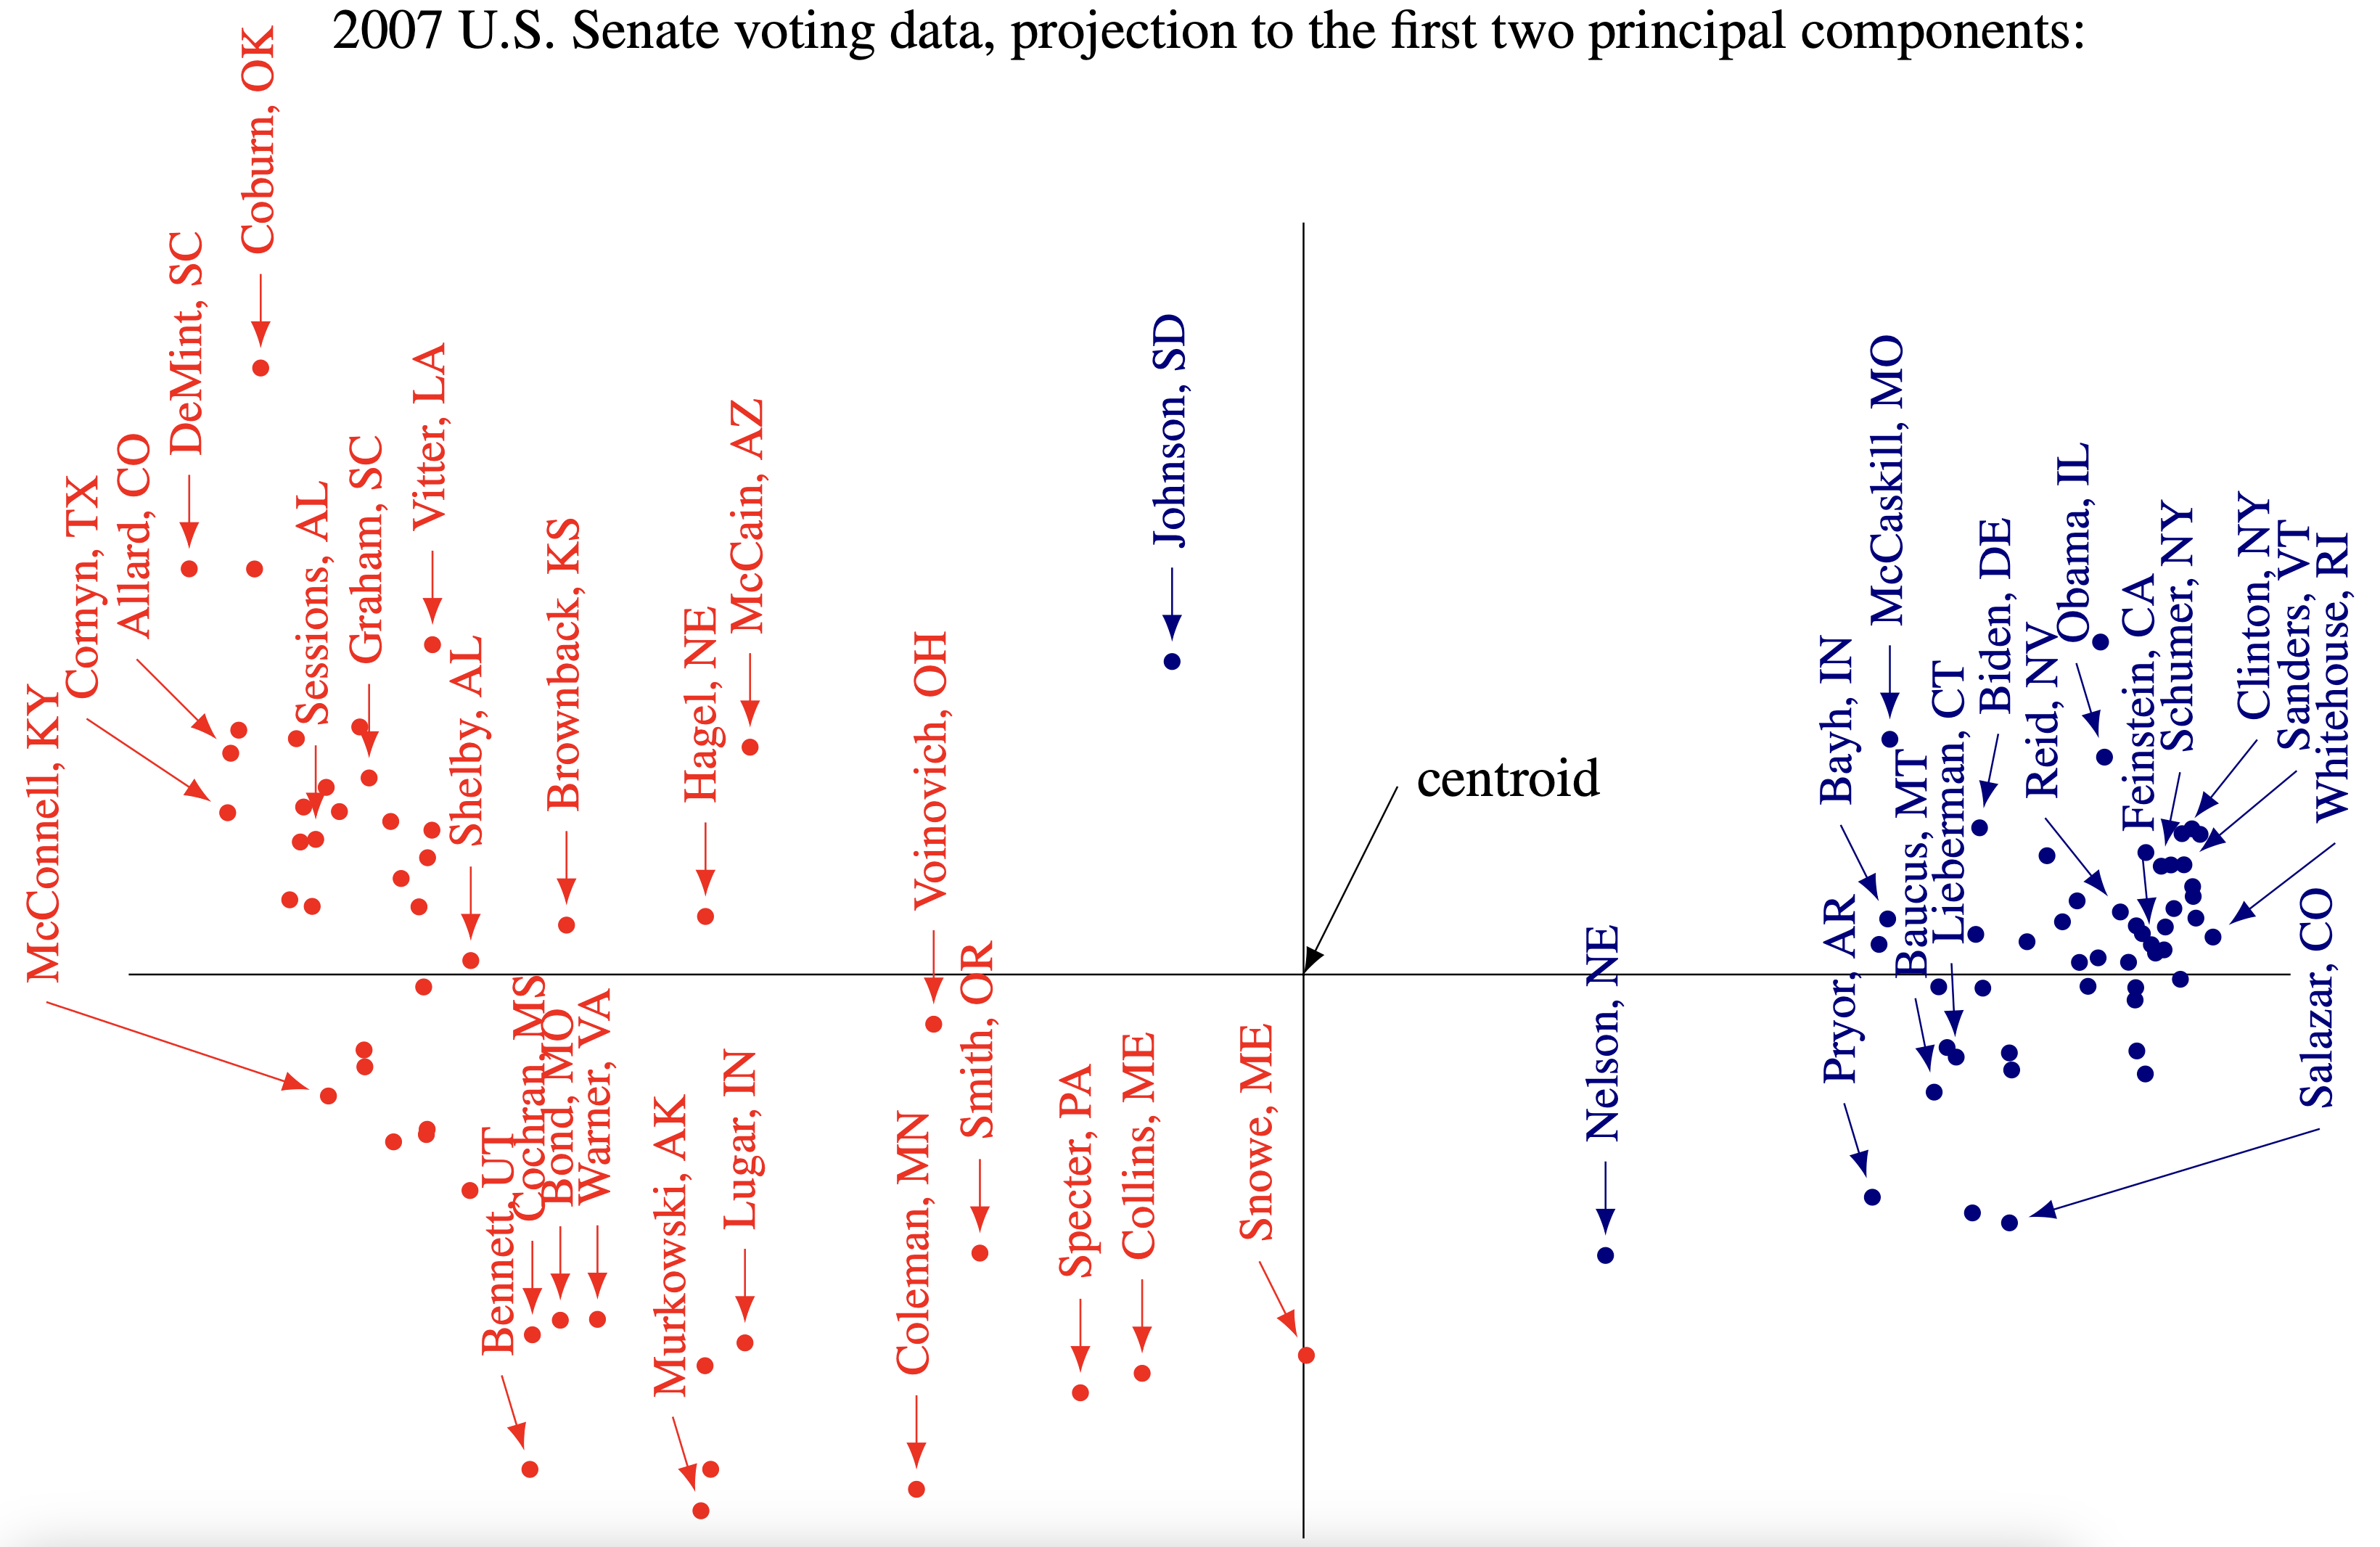
\includegraphics[width=33.06cm, height=21.49cm]{pca_senate_3.png}
\end{center}

The picture clearly shows senators clustering in certain areas. We can
use this to help answer certain questions, for example, {\em ``How
  different was Sanders's voting record from Clinton's?''}. However,
although the 2-dimensional picture seems to reveal more detail, its
interpretation is less clear. While it seems obvious that the
horizontal axis corresponds to a conservative vs.\ liberal world view,
it is much less obvious what the political meaning of the vertical
axis is. 

Maybe it is related to some issue that does not typically
follow party lines, such as North vs. South, rich states vs. poor
states, pro-immigration vs. anti-immigration, and so on.  To find a
convincing interpretation of the vertical axis, further investigation
of the data would be required (such as, looking at the actual content
of the votes in question).

The rest of the chapter will be devoted to examining how we find these useful low-dimensional subspaces that help explain data that we come across. By doing so, we'll further explore important concepts such as best-fitting subspaces, projecting onto subspaces, data spread (i.e. variance), and more.

\subsection*{Use at your own risk}
Finally, a word of caution. Whenever we use mathematics to try to draw
real-world conclusions from data, these conclusions should be taken
with an extra-large grain of salt. People have an outsized tendency to
trust mathematics and to take its results as infallible. We therefore
have a special responsibility not to overstate any conclusions, and to
point out potential pitfalls with the analysis. No matter how
wonderful principal complement analysis is, we must keep in mind that
what we are still only looking at a 2-dimensional projection of a
200-dimensional space. Therefore it is inevitable that lots of details
and nuances are lost. We could get a completely different picture by
looking at a different 2-dimensional projection.

To see how the data can sometimes be misleading, consider the question
{\em ``How similar is Senator Tim Johnson, Democrat of South Dakota,
  to Senators Olympia Snowe and Susan Collins of Maine?''}. In the
1-dimensional picture, it looked as if they were very similar. We
could easily rationalize this by pointing out that Johnson is the most
conservative Democrat, and Snowe and Collins are the most liberal
Republicans. However, the 2-dimensional picture reveals an interesting
nuance, which is that the voting records of Johnson is not all that
similar to that of Snowe and Collins. It is entirely possible that if
we add a third or fourth dimension to the picture, many more
additional such details will emerge. In summary, while principal
component analysis is a useful tool, it is just one tool among many,
and we always need to exercise our best judgement in drawing
conclusions from data.

\section*{Text Source}

This application exposition has been added to and minorly adapted from Peter Selinger's {\it Matrix Theory and Linear Algebra}, Lyrix 2018, Creative Commons License (CC-BY 4.0).
    
https://www.mathstat.dal.ca/~selinger/linear-algebra/

The referenced spreadsheet is available from
\url{https://www.mathstat.dal.ca/~selinger/linear-algebra/} under
``Supplementary materials''. Here are the first few rows and columns
of the spreadsheet.

Selinger's exposition was originally inspired by Examples~11.2.13
and 11.3.15 of {\em ``Coding the Matrix: Linear Algebra through
  Computer Science Applications''} by Philip N. Klein.


\end{document}